\documentclass{article}
\usepackage[utf8]{inputenc}
\usepackage{amsmath}
\usepackage{amsfonts}
\usepackage{tikz}

\begin{document}

\thispagestyle{empty}

\begin{figure}[htbp]
\centering
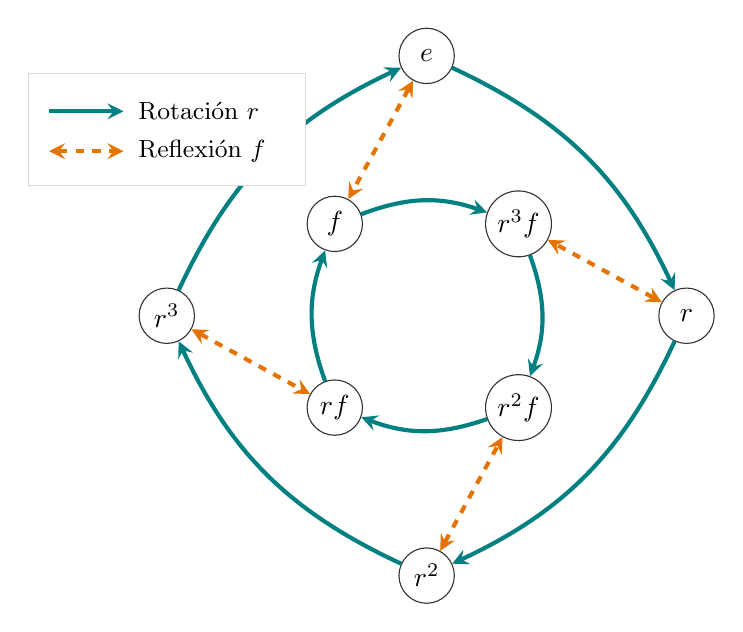
\begin{tikzpicture}[
    scale=2.2,
    % Letra un punto más grande que la original (\normalsize en lugar de \small)
    nodo/.style={circle, draw=black!80, fill=white, inner sep=2pt, minimum size=2em, font=\normalsize},
    % Grosor ligeramente mayor (1.5pt en lugar de 1.1pt)
    flechaRotacion/.style={->, >=stealth, color=teal, line width=1.5pt},
    flechaReflexion/.style={<->, >=stealth, color=orange!90!black, dashed, line width=1.5pt}
]

    % --- DEFINICIÓN DE LOS VÉRTICES ---
    % Círculo exterior (4 nodos)
    \node[nodo] (e)   at (90:1.5)   {$e$};
    \node[nodo] (r)   at (0:1.5)    {$r$};
    \node[nodo] (r2)  at (270:1.5)  {$r^2$};
    \node[nodo] (r3)  at (180:1.5)  {$r^3$};

    % Círculo interior (4 nodos)
    \node[nodo] (f)   at (135:0.75)  {$f$};
    \node[nodo] (r3f) at (45:0.75)   {$r^3 f$};
    \node[nodo] (r2f) at (315:0.75)  {$r^2 f$};
    \node[nodo] (rf)  at (225:0.75)  {$r f$};


    % --- ARISTAS DE ROTACIÓN (r) ---
    \draw[flechaRotacion] (e) to[bend left=20] (r);
    \draw[flechaRotacion] (r) to[bend left=20] (r2);
    \draw[flechaRotacion] (r2) to[bend left=20] (r3);
    \draw[flechaRotacion] (r3) to[bend left=20] (e);

    \draw[flechaRotacion] (f) to[bend left=20] (r3f);
    \draw[flechaRotacion] (r3f) to[bend left=20] (r2f);
    \draw[flechaRotacion] (r2f) to[bend left=20] (rf);
    \draw[flechaRotacion] (rf) to[bend left=20] (f);


    % --- ARISTAS DE REFLEXIÓN (f) ---
    \draw[flechaReflexion] (e) -- (f);
    \draw[flechaReflexion] (r) -- (r3f);
    \draw[flechaReflexion] (r2) -- (r2f);
    \draw[flechaReflexion] (r3) -- (rf);


    % --- LEYENDA ---
    \begin{scope}[shift={(-2.3, 1.4)}]
        \draw[fill=white, draw=gray!30] (0,0) rectangle (1.6,-0.65);
        \draw[flechaRotacion] (0.12,-0.22) -- (0.55,-0.22);
        \node[right, font=\small] at (0.58,-0.22) {Rotación $r$};
        
        \draw[flechaReflexion] (0.12,-0.45) -- (0.55,-0.45);
        \node[right, font=\small] at (0.58,-0.45) {Reflexión $f$};
    \end{scope}

\end{tikzpicture}
\end{figure}

\end{document}
